\documentclass[fontsize=10pt, twoside=no]{scrartcl} % KOMA class

% other packages %
%\usepackage{graphicx}
\usepackage{titlesec}
%\usepackage{url}
\usepackage{fancybox}

% lang : french %
\usepackage[utf8]{inputenc}
\usepackage{xspace}
\usepackage[francais]{minitoc}
\usepackage{algorithm}
\usepackage{algorithmic}
\usepackage{graphicx}
\usepackage[T1]{fontenc}
\usepackage[english,frenchb]{babel}
%\usepackage[unicode,hidelinks]{hyperref}

% mise en page %
\pagestyle{empty}
\KOMAoptions{parskip=false}
\KOMAoptions{paper=a4,DIV=22}

\addto\captionsfrench{\def\partname{}}
\renewcommand{\thepart}{}
%%%%%%%%%%%%%%

\begin{document}

\title{MLEA : SVM(Support Vector Machine)}
\author{Thibault \textsc{Lapassade} - Florian \textsc{Thomassin}}
\date{}
\maketitle
\vspace*{-3cm}

\part{}

Le but de ce rapport est de présenter les résultats de notre étude des kernel de différents SVM dans le but de déterminer le plus efficace de ces kernels. Pour cela, on distinguera deux parties :

\begin{description}
\item[Les différents kernels] qui permettra de présenter les différents types de kernel choisit et le choix des paramètres pour chacun.
\item[Le benchmark] qui permettra de présenter grâce à des graphiques les résultats de chacune de nos expérimentations sur les kernels précédemment choisis.
\end{description}

Notre système de test est réalisé à l'aide de Matlab. Le format d'entrée des données d'acquisition est fixé et n'est pas le sujet d'étude de ce compte-rendu. On s'attardera plutôt à détailler l'analyse des kernels et du choix des paramètres de ceux-ci de manière à avoir la meilleur classification.

\part{Choix des kernels et des paramètres}

Afin de pouvoir comparer les différents comportement d'un SVM en fonction du type de kernel (linear, polynomial, RBF, Laplacien RBF). De plus, nous allons faire varier le paramètre C et Gamma (si présent) pour étudier la variation de l'erreur.\\

Pour chaque type de kernel, nous allons tester les valeurs de C suivante:
\begin{itemize}
	\item C = 1
	\item C = 10
	\item C = 100
	\item C = 1000
	\item C = 10000
	\item Gamma = 2 et 4
\end{itemize}

Afin de menner a bien se benchmark, nous avons utiliser l'implementation fait en TP du SVM. Deplus, nous avons choisis le set IRIS pour faire nos tests. Possedant 3 dimentions nous avons utilisé l'algorithme DAG pour départager le SVM.\\

\noindent Nous avons définit un protocole de test suivant pour chaque kernel:
\begin{itemize}
	\item Entrainement des SVMs
	\item Tests des SVMs
	\item Application de l'algo DAG
	\item Récupération de l'erreur
	\item Création des diagrammes
\end{itemize}

\item[Kernel Linear - ] Une fois la phase test fini, nous avons constaté que les performances de ce kernel se rapprochait d'une classification aléatoire puisque le taux d'erreur  est d'environ 50\%.\\

\item[Kernel Polynomial - ] Pour ce kernel nous avons choisi le second ordre et l'ordre 4 afain d'avoir une assez grande marge pour avoir des résultats assez différents. Mais malgré ce changement d'ordre, nous avons toujours des taux d'erreurs très proches.\\

\item[Kernel Laplacian RBF - ] Nous nous sommes également aperçu que les taux d'erreurs de ce kernel n'évoluait pas énormément en fonction de la valeur de c. Néanmoins, nous avons constaté que les taux d'erreurs obtenus étaient bien meilleur que ceux avec un kernel polynomial puisque l'on divisait presque par moitié le taux d'erreur par rapport aux différents kernels polynomiaux. Nous avons ensuite testé avec un gamma de 4 de manière à voir si cela avait une influence ou non. Nous avons ainsi vue que les résultats n'étaient pas meilleurs mais au contraire plus mauvais qu'avec un gamma égale à 2.\\

\item [Kernel RBF - ] Nous avons donc mis en place un kernel RBF avec les mêmes paramètres que le Laplacian RBF. Les résultats obtenus sont identique aux précent. Néanmoins, nous nous sommes aperçu que le kernel Laplacian RBF donnait de meilleur résultat que le kernel RBF. Nous avons néanmoins aussi remarqué que certaines fois, le kernel RBF avec un gamma égale à 2 avait de moins bon résultat que le kernel RBF avec un gamma égale à 4 mais puisqu'il y avait plus de fois où le taux d'erreur est inférieur lorsque le gamma valait 2, nous nous sommes dit que cela n'était pas significatif.\\

Nous avons ensuite essayé de tester avec des kernels étant des combinaisons de kernel précedemment tester mais les temps étaient beaucoup plus grand et ne donnaient pas vraiment de meilleur résultat et donc nous avons décidé de ne pas les faire apparaître dans notre benchmark.

\part{Benchmark des kernels choisis}

\fbox{\begin{minipage}{0.9\textwidth}
\begin{center}
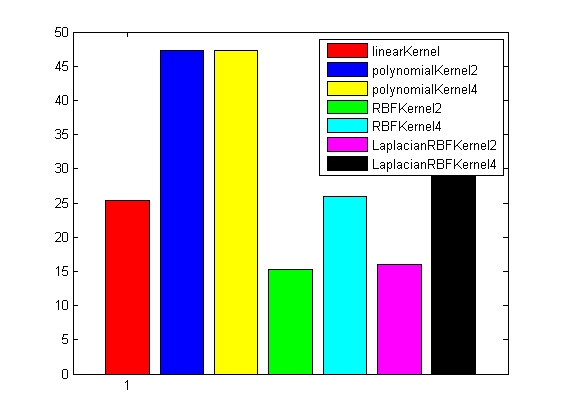
\includegraphics[scale=0.5]{image/c1.png}\\
\textsc{c = 1}\\
\end{center}
\end{minipage}}\\


\fbox{\begin{minipage}{0.9\textwidth}
\begin{center}
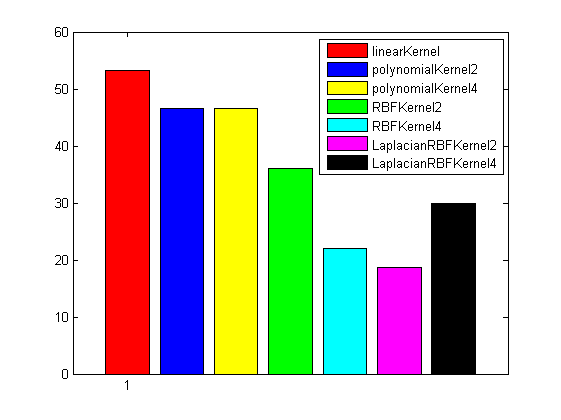
\includegraphics[scale=0.5]{image/c10.png}\\
\textsc{c = 10}\\
\end{center}
\end{minipage}}\\


\fbox{\begin{minipage}{0.9\textwidth}
\begin{center}
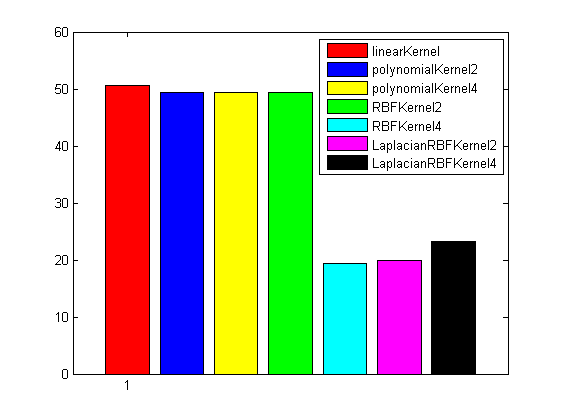
\includegraphics[scale=0.5]{image/c100.png}\\
\textsc{c = 100}\\
\end{center}
\end{minipage}}\\


\fbox{\begin{minipage}{0.9\textwidth}
\begin{center}
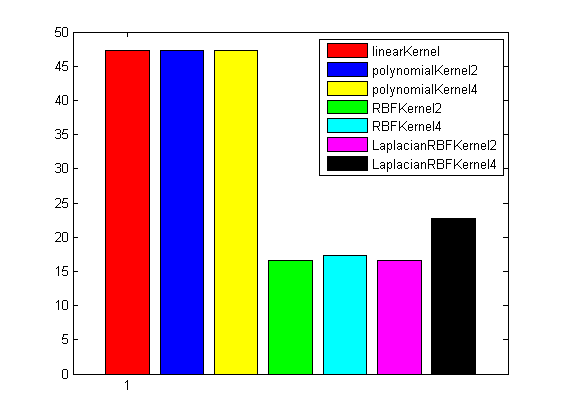
\includegraphics[scale=0.5]{image/c1000.png}\\
\textsc{c = 1000}\\
\end{center}
\end{minipage}}\\


\fbox{\begin{minipage}{0.9\textwidth}
\begin{center}
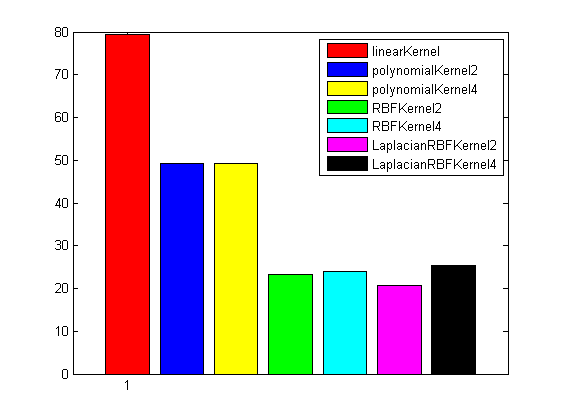
\includegraphics[scale=0.5]{image/c10000.png}\\
\textsc{c = 10000}\\
\end{center}
\end{minipage}}\\

\fbox{\begin{minipage}{0.9\textwidth}
\begin{center}
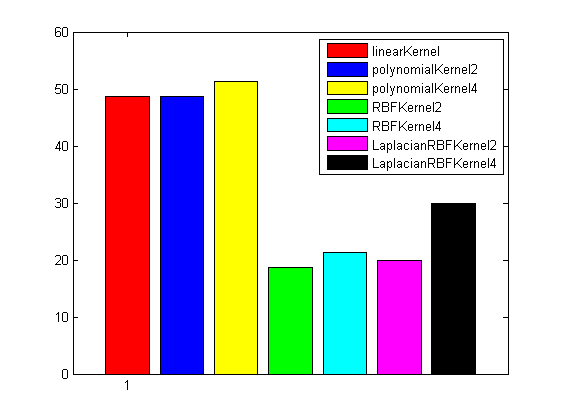
\includegraphics[scale=0.5]{image/cinf.png}\\
\textsc{c = inf}\\
\end{center}
\end{minipage}}\\

\part{Conclusion}

\`A partir des images des benchmarks précédents ainsi que grâce aux différents tests que nous avons pu effectué sur les différents kernels, on s'aperçoit que le kernel LaplacianRBF avec comme paramètre gamma=2 semble être le kernel le plus a même de bien classifier les données dont nous disposons pour le test. Néanmoins, il ne faut pas oublier que nos benchmark ont été uniquement effectué sur le set de data iris et pas sur le set de data opdigit pour cause de problème lors de l'apprentissage sur ce set et que nos résultats sont peut être biaisés par ce manque de données de test et ne reflètent donc peut être pas la réalité.


\end{document}
